\documentclass[12pt,a4paper]{article}
%\usepackage{fontspec, xunicode, xltxtra}  
%\setmainfont{Hiragino Sans GB}  
%\usepackage{xeCJK}
%\setCJKmainfont[BoldFont=STZhongsong, ItalicFont=STKaiti]{STSong}
%\setCJKsansfont[BoldFont=STHeiti]{STXihei}
%\setCJKmonofont{STFangsong}

%使用Xelatex编译

% 设置页面
%==================================================
\linespread{2} %行距
% \usepackage[top=1in,bottom=1in,left=1.25in,right=1.25in]{geometry}
% \headsep=2cm
% \textwidth=16cm \textheight=24.2cm
%==================================================

% 其它需要使用的宏包
%==================================================
\usepackage[colorlinks,linkcolor=blue,anchorcolor=red,citecolor=green,urlcolor=blue]{hyperref} 
\usepackage{tabularx}
\usepackage{authblk}         % 作者信息
\usepackage{algorithm}     % 算法排版
\usepackage{amsmath}     % 数学符号与公式
\usepackage{amsfonts}     % 数学符号与字体
\usepackage{mathrsfs}      % 花体
\usepackage{amssymb}
\usepackage[framemethod=TikZ]{mdframed}

\usepackage{graphicx} 
\usepackage{graphics}
\usepackage{color}
\usepackage{xcolor}
\usepackage{tcolorbox}
\usepackage{lipsum}

\usepackage{fancyhdr}       % 设置页眉页脚
\usepackage{fancyvrb}       % 抄录环境
\usepackage{float}              % 管理浮动体
\usepackage{geometry}     % 定制页面格式
\usepackage{hyperref}       % 为PDF文档创建超链接
\usepackage{lineno}          % 生成行号
\usepackage{listings}        % 插入程序源代码
\usepackage{multicol}       % 多栏排版
%\usepackage{natbib}         % 管理文献引用
\usepackage{rotating}       % 旋转文字,图形,表格
\usepackage{subfigure}    % 排版子图形
\usepackage{titlesec}       % 改变章节标题格式
\usepackage{moresize}   % 更多字体大小
\usepackage{anysize}
\usepackage{indentfirst}  % 首段缩进
\usepackage{booktabs}   % 使用\multicolumn
\usepackage{multirow}    % 使用\multirow

\usepackage{wrapfig}
\usepackage{titlesec}     % 改变标题样式
\usepackage{enumitem}
\usepackage{aas_macros}

\newcommand{\myvec}[1]%
   {\stackrel{\raisebox{-2pt}[0pt][0pt]{\small$\rightharpoonup$}}{#1}}  %矢量符号
\renewcommand{\vec}[1]{\boldsymbol{#1}}
\newcommand{\me}{\mathrm{e}}
\newcommand{\mi}{\mathrm{i}}
\newcommand{\dif}{\mathrm{d}}
\newcommand{\tabincell}[2]{\begin{tabular}{@{}#1@{}}#2\end{tabular}}

\def\kpc{{\rm kpc}}
\def\km{{\rm km}}
\def\cm{{\rm cm}}
\def\TeV{{\rm TeV}}
\def\GeV{{\rm GeV}}
\def\MeV{{\rm MeV}}
\def\GV{{\rm GV}}
\def\MV{{\rm MV}}
\def\yr{{\rm yr}}
\def\s{{\rm s}}
\def\ns{{\rm ns}}
\def\GHz{{\rm GHz}}
\def\muGs{{\rm \mu Gs}}
\def\arcsec{{\rm arcsec}}
\def\K{{\rm K}}
\def\microK{\mu{\rm K}}
\def\sr{{\rm sr}}
\newcolumntype{p}{D{,}{\pm}{-1}}

\renewcommand{\figurename}{Fig.}
\renewcommand{\tablename}{Tab.}

\renewcommand{\arraystretch}{1.5}

\setlength{\parindent}{0pt}  %取消每段开头的空格

\newcounter{theo}[section]\setcounter{theo}{0}
\renewcommand{\thetheo}{\arabic{section}.\arabic{theo}}
\newenvironment{theo}[2][]{%
\refstepcounter{theo}%
\ifstrempty{#1}%
{\mdfsetup{%
frametitle={%
\tikz[baseline=(current bounding box.east),outer sep=0pt]
\node[anchor=east,rectangle,fill=blue!20]
{\strut Theorem~\thetheo};}}
}%
{\mdfsetup{%
frametitle={%
\tikz[baseline=(current bounding box.east),outer sep=0pt]
\node[anchor=east,rectangle,fill=blue!20]
{\strut Theorem~\thetheo:~#1};}}%
}%
\mdfsetup{innertopmargin=10pt,linecolor=blue!20,%
linewidth=2pt,topline=true,%
frametitleaboveskip=\dimexpr-\ht\strutbox\relax
}
\begin{mdframed}[]\relax%
\label{#2}}{\end{mdframed}}




\title{Equilibria of Collisionless Systems}
\author{}
\date{\today}
\begin{document}

\maketitle

\cite{2008gady.book.....B}  The stellar systems may be considered to be collisionless. A good approximation to the orbit of any star can be obtained if the system's mass were smoothly distributed in space rather than concentrated into nearly point-like stars. Eventually, the true orbit deviates significantly from this model orbit, but in systems with more than a few thousand stars, the deviation is small for a time $\lesssim t_{\rm relax}$ that is much larger than the crossing time $t_{\rm cross}$. For a galaxy, $t_{\rm relax}$ is usually much larger even than the age of the universe, so the approximation that the potential is smooth provides a complete description of the dynamics. We assume throughout that the stellar systems consist of $N$ identical point masses, which might be stars or dark-matter particles.

\section{The collisionless Boltzmann equation}
Introduce the probability of finding a star in the six-dimensional phase-space volume $\dif^3 \vec{x} \dif^3 \vec{v}$ around the position $\vec{x}$ and velocity $\vec{v}$. Define the distribution function (DF) $f$ such that $f(\vec{x}, \vec{v}, t) \dif^3 \vec{x} \dif^3 \vec{v}$ is the probability that at time $t$ a randomly chosen star, say star $1$, has phase-space coordinates in the given range. $f$ is normalized
\begin{equation}
\int f(\vec{x}, \vec{v}, t) \dif^3 \vec{x} \dif^3 \vec{v} = 1 ~,
\end{equation}
where the integral is over all phase space. Let $\vec{w} = (\vec{x}, \vec{v})$ be the usual Cartesian coordinates, and consider an arbitrary  region $\mathcal V$ of phase space. The probability of finding star $1$ in $\mathcal V$ is $P = \int_{\mathcal V} \dif^6 \vec{w} f(\vec{w})$. Let $\vec{W}$ represent some arbitrary set of phase-space coordinates,  and let $F(\vec{W})$ be the corresponding DF. That is the probability of finding star $1$ in $\mathcal V$ is $P = \int_{\mathcal V} \dif^6 \vec{W} F(\vec{W})$. If $\mathcal V$ is small enough, $f$ and $F$ will be approximately constant throughout it, and we can take them outside the integrals for $P$. Thus
\begin{equation}
P = f(\vec{w}) \int_{\mathcal V} \dif^6 \vec{w} = F(\vec{W}) \int_{\mathcal V} \dif^6 \vec{W} 
\end{equation}
If the coordinates $\vec{W}$ are canonical, $\int_{\mathcal V} \dif^6 \vec{w} = \int_{\mathcal V} \dif^6 \vec{W}$. Therefore $f(\vec{w}) = F(\vec{W})$, i.e. the DF has the same numerical value at a given phase-space point in any canonical coordinate system. This invariance enables us to treat $\vec{w} = (\vec{q}, \vec{p})$ as an arbitrary system of canonical coordinates.

Any given star moves through phase space, so the probability of finding it at any given phase-space location evolves with time. As $f$ evolves, probability must be conserved, 
\begin{equation}
\frac{\partial f}{\partial t} +\frac{\partial }{\partial \vec{w}}\cdot (f \dot{\vec{w}}) ~.
\end{equation}
According to the Hamilton's equations, the second term is
\begin{eqnarray}
\nonumber \frac{\partial }{\partial \vec{q}}\cdot (f \dot{\vec{q}}) +\frac{\partial }{\partial \vec{p}}\cdot (f \dot{\vec{p}}) &=& \frac{\partial }{\partial \vec{q}}\cdot \left(f \frac{\partial H}{\partial \vec{p}} \right) +\frac{\partial }{\partial \vec{p}}\cdot \left(f \frac{\partial H}{\partial \vec{q}} \right) \\
\nonumber &=& \frac{\partial f}{\partial \vec{q}}\cdot \frac{\partial H}{\partial \vec{p}} -\frac{\partial f}{\partial \vec{p}} \cdot \frac{\partial H}{\partial \vec{q}} \\
&=& \dot{\vec{q}} \cdot \frac{\partial f}{\partial \vec{q}}+ \dot{\vec{p}}\cdot \frac{\partial f}{\partial \vec{p}}
\end{eqnarray}
Then the collisionless Boltzmann equation is
\begin{equation}
\frac{\partial f}{\partial t} +\dot{\vec{q}} \cdot \frac{\partial f}{\partial \vec{q}}+ \dot{\vec{p}}\cdot \frac{\partial f}{\partial \vec{p}} = \frac{\partial f}{\partial t} +\frac{\partial f}{\partial \vec{q}}\cdot \frac{\partial H}{\partial \vec{p}} -\frac{\partial f}{\partial \vec{p}}\cdot \frac{\partial H}{\partial \vec{q}} = \frac{\partial f}{\partial t} + [f, H] = 0 ~,
\end{equation}
where the square bracket is a Poisson bracket.

Define 
\begin{equation}
\frac{\dif f}{\dif t} \equiv \frac{\partial f}{\partial t} +\dot{\vec{w}} \cdot \frac{\partial f}{\partial \vec{w}}
\end{equation}
where $\dfrac{\dif f}{\dif t}$ represents the rate of change of the local probability density as seen by an observer who moves through phase space with a star. Since
\begin{equation}
\dot{\vec{w}} \cdot \frac{\partial f}{\partial \vec{w}} = [f, H] ~,
\end{equation}
\begin{equation}
\frac{\dif f}{\dif t} = \frac{\partial f}{\partial t} +[f, H] = 0 ~,
\end{equation}
The flow through phase space of the probability fluid is incompressible. The phase-space density $f$ of the fluid around a given star always remains the same. In contrast to flows of incompressible fluids such as water, the density will generally vary greatly from point to point in phase space. The density is constant as one follows the flow around a particular star but the density around different stars can be quite different.

In inertial Cartesian coordinates, $H = \dfrac{v^2}{2} + \Phi(\vec{x}, t)$ with $\Phi$ the gravitational potential, the collisionless Boltzmann equation is
\begin{equation}
\frac{\partial f}{\partial t} +\vec{v} \cdot \frac{\partial f}{\partial \vec{x}} -\frac{\partial \Phi}{\partial \vec{x}}\cdot \frac{\partial f}{\partial \vec{v}} = 0 ~.
\end{equation}
In cylindrical coordinates, $H = \dfrac{ (p_R^2 +p_\phi^2/R^2 +p_z^2) }{2}+\Phi$, the collisionless Boltzmann equation becomes
\begin{equation}
\frac{\partial f}{\partial t} +p_R \frac{\partial f}{\partial R} +\frac{p_\phi}{R^2} \frac{\partial f}{\partial \phi} +p_z \frac{\partial f}{\partial z} -\left(\frac{\partial \Phi}{\partial R} -\frac{p^2_\phi}{R^3} \right)\frac{\partial f}{\partial p_R} -\frac{\partial \Phi}{\partial \phi} \frac{\partial f}{\partial p_\phi} -\frac{\partial \Phi}{\partial z} \frac{\partial f}{\partial p_z} = 0
\end{equation}
In spherical polar coordinates, $H = \dfrac{1}{2}\left(p_r^2 +\dfrac{p_\theta^2}{r^2} +\dfrac{p_\phi^2}{r^2 \sin^2 \theta} \right) + \Phi(\vec{x}, t)$, and
\begin{equation}
\frac{\partial f}{\partial t} +
\end{equation}

\subsection{Limitations of the collisionless Boltzmann equation}
\subsubsection{Finite stellar lifetimes}
The physical basis of the collisionless Boltzmann equation is conservation of the objects that are described by the DF. Because stars are born and die, their flow through phase space would be described by
\begin{equation}
\frac{\dif f}{\dif t} = \frac{\partial f}{\partial t} +\vec{v} \cdot \frac{\partial f}{\partial \vec{x}} -\frac{\partial \Phi}{\partial \vec{x}}\cdot \frac{\partial f}{\partial \vec{v}} = B -D ~,
\end{equation}
where $B(\vec{x}, \vec{v}, t)$ and $D(\vec{x}, \vec{v}, t)$ are the rates per unit phase-space volume at which stars are born and die. $\vec{v} \cdot \dfrac{\partial f}{\partial \vec{x}}$ is of order $vf/R$, where $v$ and $R$ are the characteristic speed and radius in the galaxy. The ratio $R/v$ is simply the crossing time $t_{\rm cross}$. $\dfrac{\partial \Phi}{\partial \vec{x}}$ is of order the characteristic acceleration $a$, so the term $\dfrac{\partial \Phi}{\partial \vec{x}}\cdot \dfrac{\partial f}{\partial \vec{v}}$ is of order $\dfrac{af}{v}$. Since $a \approx \dfrac{v}{t_{\rm cross}}$, the two terms are of order $\dfrac{f}{t_{\rm cross}}$. Consider the ratio
\begin{equation}
\gamma = \Bigg| \frac{B-D}{f/t_{\rm cross}} \Bigg| ~.
\end{equation}
The collisionless Boltzmann equation is valid if $\gamma \ll 1$, which requires that the fractional change in the number of stars per crossing time is small.




\subsubsection{Correlations between stars}
The average number density of stars in an infinitesimal volume of phase space is $Nf$. The density is $N \bar{f}$, where $\bar{f}$ is the average of $f$ within this volume. This function is sometimes called the coarse-grained DF. The standard df is then called the fine-grained DF. However, this assumption will only be correct if the positions of stars in phase space are uncorrelated: that is, knowing that star $1$ is at $\vec{w}$ makes it neither more nor less likely that another star, say star $2$, is at an adjacent phase-space location $\vec{w}^\prime$, i.e. the probability of finding star $1$ in the volume $\dif^6 \vec{w}$ at $\vec{w}$ and star $2$ in $\dif^6 \vec{w}^\prime$ at $\vec{w}^\prime$ is simply the product $f(\vec{w}) \dif^6 \vec{w} f(\vec{w}^\prime) \dif^6 \vec{w}^\prime$ of the probabilities of finding star $1$ at $\vec{w}$ and star $2$ at $\vec{w}^\prime$. The distributions are ``separable". When the assumption of separability holds, the probability $P_{\mathcal V}(k)$ that we will find $k$ stars in a given volume $\mathcal V$ of phase space is given by the Poisson distribution 
\begin{equation}
P_{\mathcal V}(k) = \frac{\mu^k}{k!} e^{-\mu} 
\end{equation}
where
\begin{equation}
\mu \equiv N \bar{f} \mathcal V
\end{equation}
The mean number of stars predicted by this probability distribution is $\langle k \rangle = N \bar{f} \mathcal V$. $N\bar{f}$ is the expectation value of the stellar number density, if the DF is separable. Two obvious corollaries are that the mean mass within $\mathcal V$ is
\begin{equation}
\langle m \rangle = M \bar{f}(\vec{w}) \mathcal V
\end{equation}
where $M$ is the total mass of the stellar system, and the mean luminosity emitted within $\mathcal V$ is
\begin{equation}
\langle l \rangle = L \bar{f}(\vec{w}) \mathcal V
\end{equation}
where $L$ is the system's luminosity.

In reality, the presence of star $1$ at $\vec{x}$ always increases the probability that star $2$ will be found at some nearby position $\vec{x}^\prime$ because stars attract one another.


\subsubsection{Relation between the DF and observables}
At any fixed position $\vec{x}$, the integral
\begin{equation}
\nu(\vec{x}) \equiv \int \dif^3 \vec{v} f(\vec{x}, \vec{v}) ~,
\end{equation}
gives the probability per unit volume of finding a particular star at $\vec{x}$, regardless of its velocity. The real-space number density of stars is obtained by multiplying the total number $N$ of stars in the population,
\begin{equation}
n(\vec{x}) \equiv N\nu(\vec{x}) ~.
\end{equation}
In the Galaxy $n(\vec{x})$ can in principle be determined from star counts, and thus $\nu(\vec{x})$ can be derived from $n(\vec{x})$. In other galaxies it is not usually possible to count stars, but we can derive $\nu(\vec{x})$ from the luminosity density $j(\vec{x}) = L\nu(\vec{x})$, where $L$ is the luminosity of the stellar population.






















\section{Jeans theorems}
A function of the phase-space coordinates $I(\vec{x}, \vec{v})$ is an integral if and only if
\begin{equation}
\frac{\dif I[\vec{x}(t), \vec{v}(t)]}{\dif t} = 0
\end{equation}
along any orbit. With the equations of motion, this becomes
\begin{eqnarray*}
\frac{\dif I}{\dif t} = \frac{\partial I}{\partial \vec{x} } \cdot  \frac{\dif\vec{x}}{\dif t}  +\frac{\partial I}{\partial \vec{v} } \cdot  \frac{\dif\vec{v}}{\dif t} = 0 ~, {\rm or }\\
\vec{v} \cdot \frac{\partial I}{\partial \vec{x} } -\frac{\partial \Phi}{\partial \vec{x}}\cdot \frac{\partial I}{\partial \vec{v}} = 0
\end{eqnarray*}
The condition for $I$ to be an integral is identical with the condition for $I$ to be a steady-state solution of the collisionless Boltzmann equation.
\begin{tcolorbox}[colback=green!5,colframe=green!40!black,title=Jeans theorem]
Any steady-state solution of the collisionless Boltzmann equation depends on the phase-space coordinates only through integrals of motion in the given potential, and any function of the integrals yields a steady-state solution of the collisionless Boltzmann equation.
\end{tcolorbox}
%\begin{theo}[Jeans theorem]{}
%Any steady-state solution of the collisionless Boltzmann equation depends on the phase-space coordinates only through integrals of motion in the given potential, and any function of the integrals yields a steady-state solution of the collisionless Boltzmann equation.
%\end{theo}
Proof : 
































If all orbits in a galaxy are regular, then we can forget about any non-isolating integrals.
\begin{tcolorbox}[colback=green!5,colframe=green!40!black,title=Strong Jeans theorem]
The df of a steady-state stellar system in which almost all orbits are regular with non-resonant frequencies may be presumed to be a function only of three independent isolating integrals, which may be taken to be the actions.
\end{tcolorbox}




\section{Collisionless Dynamics}
\cite{2010gfe..book.....M}


\section{Collisionless Relaxation}
\cite{2010gfe..book.....M} In dynamics, relaxation is the process by which a system approaches equilibrium or by which it returns to equilibrium after a disturbance. 

The range of equilibrium configurations accessible to a collisionless system is extremely large. Yet galaxies only seem to occupy a relatively small volume of this configuration space, as is evident from the fact that galaxies obey a number of relatively tight scaling relations, and have a fairly restricted variety of density profiles. 

For an isolated gas, it is well known that the collisions and interactions among the gas particles cause the system to relax to a Maxwellian distribution characterized by a single temperature. During this relaxation process most information regarding the initial conditions is erased. In the case of a collisionless system, however, the two-body relaxation time is much longer than the Hubble time, so that two-body interactions cannot be the main relaxation mechanism. A collisionless system obeys the collisionless Boltzmann equation (CBE), which also remains valid during the gravitational collapse.

Defined $f(\vec{x}, \vec{v})$ as the number density of particles. On infinitesimally small scales the distribution of particles becomes a sum of Dirac delta functions, so that the DF can no longer be considered as a smooth density field in phase space, and the CBE becomes ill-defined. $f$ is a probability function, with $f(\vec{x}, \vec{v}) \dif \vec{x} \dif \vec{v}$ the probability of finding a particle in the phase-space volume ($\vec{x} \pm \dif \vec{x}/2$, $\vec{v} \pm \dif \vec{v}/2$). Although this probability function is well-defined, with its evolution governed by the CBE, it is not directly measurable. Rather, an observer can only measure the numbers of stars in finite phase-space volume elements. The corresponding DF, \textcolor{red}{$f_c(\vec{x},\vec{v})$}, is called the \textcolor{red}{coarse-grained distribution function}\footnote{\textcolor{red}{$f$} is called the \textcolor{red}{fine-grained distribution function}.}, and corresponds to the \textcolor{orange}{average of $f(\vec{x},\vec{v})$ in some phase-space volume element centered on $(\vec{x},\vec{v})$}. Contrary to $f$, the \textcolor{yellow}{coarse-grained DF does not obey the CBE}. However, if \textcolor{red}{$\partial f_c/\partial t = 0$}, then the system will appear relaxed to an observer, as it does not reveal any observable evolution. Thus, as a working definition we may refer to relaxation as the process that drives the system towards a state with $\partial f_c/\partial t \simeq 0$.

There are four different relaxation mechanisms at work in gravitational $N$-body systems: phase mixing, chaotic mixing, violent relaxation and Landau damping.

\subsection{Phase Mixing}
\cite{2010gfe..book.....M} Consider two regular orbits with similar values for the actions $J_i$, i.e. whose tori are similar and close to each other in phase space. Since the fundamental frequencies are functions of the actions, they will also be similar for the two orbits. Consider two trajectories on these two tori that initially have similar phases (i.e. the two trajectories are initially close to each other in phase space). Since the fundamental frequencies of the two trajectories are similar but not identical, the trajectories will separate. In particular, the phase difference in direction $i$ will increase with time according to $\Delta \phi_i(t) = 2\pi (\Delta \omega_i)t$. Thus, points that are initially close to each other in phase space will separate linearly with time, a process called \textcolor{red}{phase mixing}. The points that initially occupy the same small region in phase space are sheared out, and eventually become tightly wound. Note that during this process the fine-grained DF remains constant. However, the coarse-grained DF, measured at the location of the initial phase-space region initially decreases with time, as more and more `vacuum' (i.e. unoccupied phase-space volume) is mixed in. At some point, however, depending on the coarseness used to measure $f_c$, the coarse-grained DF will stop evolving. Hence phase mixing is a relaxation process. Note, though, information is lost only through the coarse-graining. At the fine-grained level phase mixing (and indeed all relaxation described purely by the coupled CBE and Poisson equations) is reversible and preserves all knowledge of the initial conditions.

For a system of fixed mass, the maximum of the coarse-grained DF, $f_{c, \rm max}$, cannot increase with time. Prior to reaching a relaxed state, phase mixing always continues to mix in more and more `vacuum'. This consequence of phase mixing can be used to constrain the nature of the dark matter and the formation process of galaxies.  

The time scale for phase mixing is not well defined. It basically depends on the range of (fundamental) frequencies covered by the group of particles under consideration. Note, however, that the time scale is never less than a dynamical time and can be much longer. For trajectories confined to the same torus the time scale is infinite, and no phase mixing occurs.

%===========================================================================================================================
\begin{figure*}
\centering
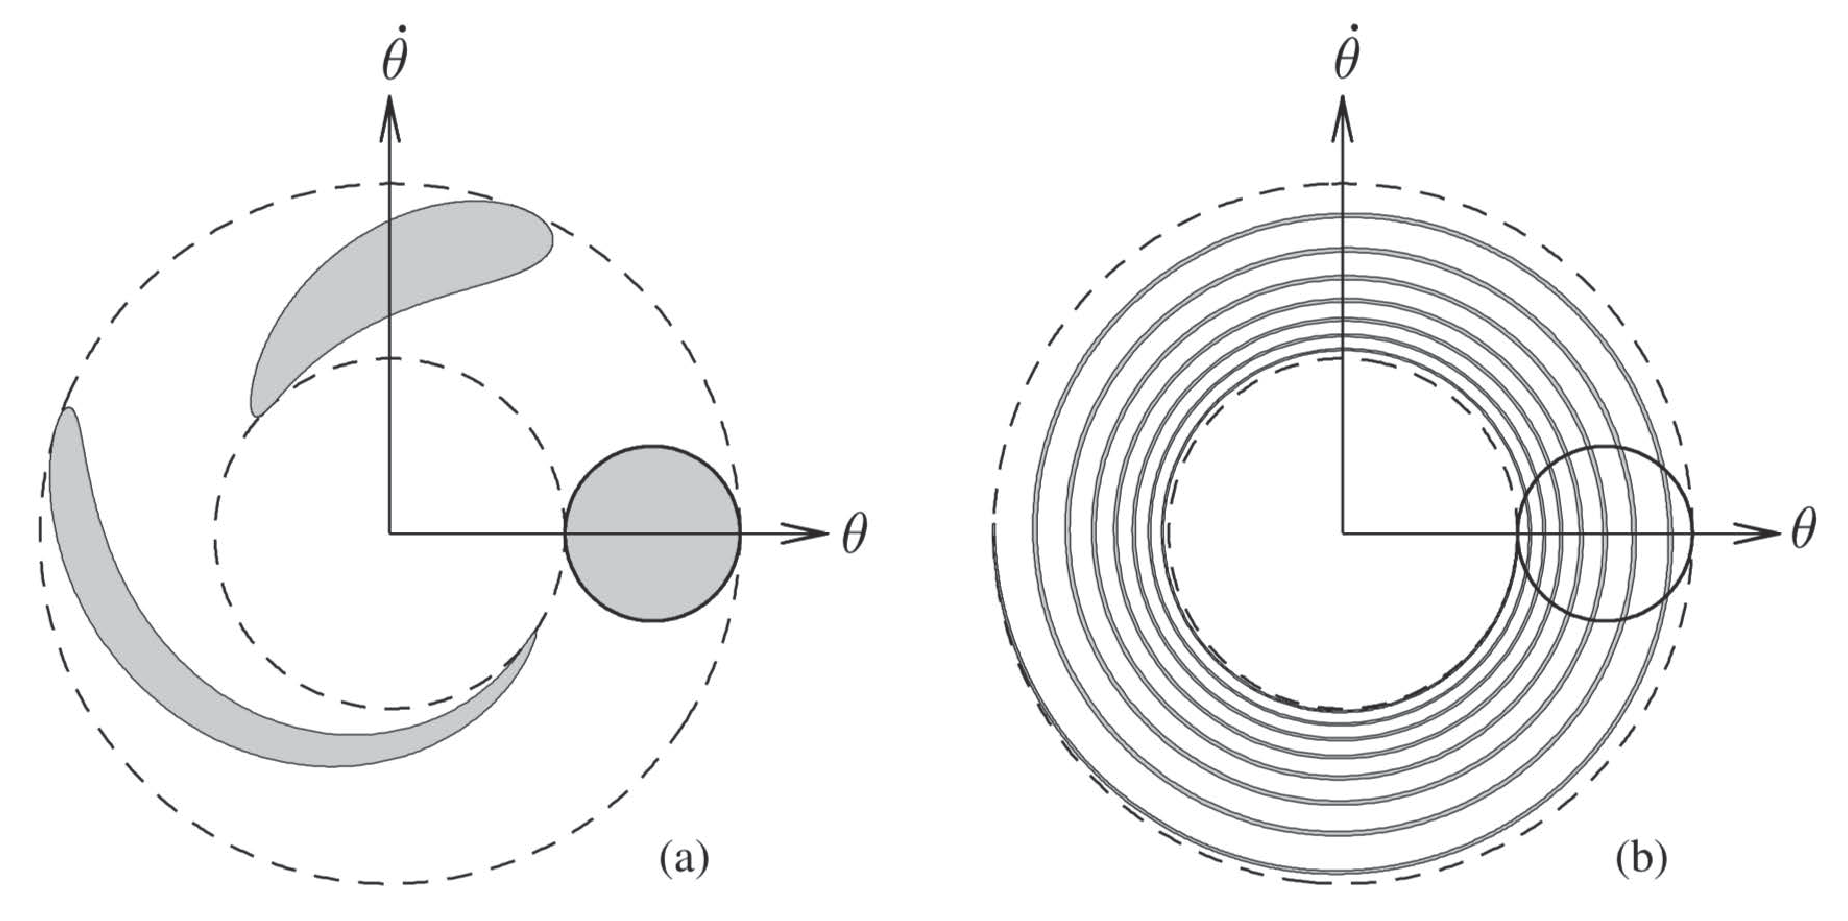
\includegraphics[height=7.cm, angle=0]{phase_mixing.eps}
\caption{
An illustration of phase mixing. Here particles are assumed to orbit in a simple one-dimensional potential. Each dashed circle in phase space represents an orbit of given energy $(\theta^2 + \dot{\theta}^2 = \text{const}.)$. The shaded circle in the phase-space diagram on the left represents a group of particles that initially occupy a small region in phase space. Since ‘orbits’ with a larger amplitude are assumed to have longer periods, this particle cloud shears as it evolves (as in a), and eventually becomes tightly wound (as in b).
}
\label{fig:homopolar}
\end{figure*}
%===========================================================================================================================

\subsection{Chaotic Mixing}
\cite{2010gfe..book.....M} While regular orbits experience phase mixing, stochastic orbits experience chaotic mixing. A characteristic property of stochastic orbits is that two stochastic trajectories that are initially close to each other diverge exponentially. A group of stars that are initially close to each other in a stochastic region of phase space will mix by spreading through the `Arnold web', the phase-space region accessible to every stochastic trajectory of given energy in a system with three degrees of freedom. After a sufficiently long time they will uniformly cover the Arnold web which implies that $\partial f_c/\partial t = 0$. As phase mixing, chaotic mixing thus smooths out (i.e. relaxes) the coarse-grained DF, but leaves the fine-grained DF invariant.

Consider two trajectories $\Gamma_1$ and $\Gamma_2$ that at some time $t_0$ pass close to some point $(\vec{x},\vec{v})$ in phase space, and let $\Delta L_i(t)$ (with $i = 1, \cdots, 2n$) indicate the distance between $\Gamma_1$ and $\Gamma_2$ in phase-space coordinate $i$ at time $t$. The Lyapunov exponents for $(\vec{x},\vec{v})$ are defined as
\begin{equation}
\lambda_i = \lim_{t \rightarrow \infty} \frac{1}{t} \ln \left(\dfrac{\dif L_i(t)}{\dif L_i(t_0)} \right) ~.
\end{equation}
In a collisionless system
\begin{equation}
\sum_{i=1}^{2n} \lambda_i = 0 ~,
\end{equation}
which expresses the incompressibility of the flow (i.e. the fact that $\dif f /\dif t = 0$). If the trajectory through $(\vec{x},\vec{v})$ is regular then $L_i(t) \propto t$, so that $\lambda_i = 0$ for all $i$. However, if the trajectory is stochastic then $\lambda \equiv {\rm max}\{\lambda_i\} > 0$, which implies that two trajectories near $(\vec{x},\vec{v})$ will diverge exponentially as $\delta \Gamma(t) \propto {\rm e}^{\lambda t}$. The inverse of the largest Lyapunov exponent is called the \textcolor{red}{Lyapunov time}, and defines the characteristic $e$-folding time for chaotic mixing, which is \textcolor{yellow}{typically much shorter than the time scale for phase mixing}. Note, though, that the actual mixing rate of stochastic ensembles typically falls below the Lyapunov rate once the trajectories separate. This reflects the fact that stochastic regions are often bounded by regular tori, which can confine stochastic orbits for long periods of time to restricted parts of phase space. The time scale on which an orbit uniformly spreads over its accessible phase-space volume then becomes dependent on the efficiency of Arnold diffusion, which can be very low.

Note that, just like phase mixing, chaotic mixing is reversible at the fine-grained level, but that the exponential divergence of neighboring trajectories means that almost infinitely precise knowledge of the phase-space structure is required to undo its effects. Hence, \textcolor{orange}{chaotic mixing effectively erases knowledge of the initial conditions much more rapidly than phase mixing}. On the other hand, while phase mixing operates in almost all collisionless systems, \textcolor{orange}{chaotic mixing is only important if a significant fraction of phase space is occupied by chaotic orbits}.

\subsection{Violent Relaxation}
\cite{2010gfe..book.....M} Phase mixing and chaotic mixing are two relaxation processes that occur even when the gravitational potential associated with the dynamical system is constant. During these relaxation processes the energies of the individual particles are conserved. However, the collapse or disturbance of a collisionless system is generally accompanied with changes of the gravitational potential, $\Phi(\vec{x},t)$, giving rise to an additional relaxation process.

Let $\varepsilon = \dfrac{1}{2} v^2 + \Phi$ be the specific energy for a given particle. 
\begin{align}
\nonumber \dfrac{\dif \varepsilon}{\dif t} &= \dfrac{\partial \varepsilon}{\partial t} \cdot \dfrac{\dif \vec{v}}{\dif t} + \dfrac{\partial \varepsilon}{\partial \Phi} \cdot \dfrac{\dif \Phi}{\dif t} = -\vec{v} \cdot \nabla \Phi + \dfrac{\dif \Phi}{\dif t} \\
&= -\vec{v} \cdot \nabla \Phi + \dfrac{\partial \Phi}{\partial t} + \vec{v} \cdot \nabla \Phi = \dfrac{\partial \Phi}{\partial t} ~,
\end{align}
where $\dfrac{\dif \vec{v}}{\dif t}) = -\nabla \Phi$. A time-dependent potential of a collisionless system can induce a change in the energies of the particles involved (i.e. in a time-varying potential, energy is no longer an integral of motion). Exactly how the energy of a particle changes depends in a complex way on the initial position and energy of the particle: in fact, particles can both gain or lose energy, and some particles can even become unbound. Overall, the effect is to broaden the range of energies. In this respect, a time-varying potential provides an additional relaxation mechanism, which is called \textcolor{red}{violent relaxation}. Note that violent relaxation still obeys the CBE, $\dif f /\dif t = 0$; however, unlike for a steady state system, the Eulerian time derivative $\partial f/\partial t \neq 0$. Furthermore, unlike phase mixing and chaotic mixing in a static potential, violent relaxation causes `mixing' of particles also in binding energy.


$\dfrac{\dif \varepsilon}{\dif t}$ is independent of particle mass, so violent relaxation has no tendency to segregate particles of differing mass during the relaxation process. This is different from collisional relaxation, where the momentum exchange associated with the two-body gravitational encounters drives the system towards equipartition of kinetic energy. More massive particles tend to transfer energy to their lighter neighbors and so become more tightly bound, sinking towards the center of the gravitational potential. This effect is known as mass segregation and is particularly important in the evolution of globular star clusters.

It is important to realize that a time-varying potential does not guarantee violent relaxation. One can construct oscillating models exhibiting no tendency to relax by making sure that no mixing occurs. In this case, the energies of the individual particles change with time, but the relative distribution of energies is invariant. Although unrealistically artificial, this demonstrates that violent relaxation requires both a time-varying potential and mixing to occur simultaneously.

The time scale for violent relaxation can be defined as
\begin{equation}
t_{\rm vr} = \left\langle \dfrac{1}{\varepsilon^2} \left( \dfrac{\partial \Phi}{\partial t} \right)^2 \right\rangle^{-1/2} ~,
\end{equation}
where the average $\langle \cdots \rangle$ is over all particles that make up the collective potential. It is approximately equal to the free-fall time\footnote{The free-fall time is the characteristic time that it would take for a body to collapse under its own gravitational attraction, if no other forces existed to oppose the collapse.} of the system, $t_{\rm ff} = (3\pi /32G \bar{\rho})^{1/2}$, with $\bar{\rho}$ the average density. This indicates that the relaxation process is very fast (hence `violent').

Like phase mixing and chaotic mixing, violent relaxation tends to erase a system's memory of its initial conditions. However, the mixing associated with violent relaxation is self-limiting, because as soon as a system approaches any equilibrium state, the large-scale potential fluctuations which drive the evolution vanish. Mixing destroys the coherent motions required to maintain these variations, for example, in the later phases of the collapse of a system or the merger of two systems. As a result it is difficult to predict the extent to which the properties of the initial conditions are reflected in the final equilibrium state. Numerical simulations have shown that violent relaxation is, in general, never `complete', in the sense that the final energies of particles are correlated with their initial values and the shape of the final system clearly remembers that of the initial conditions.


\subsection{Landau Damping}
\cite{2010gfe..book.....M} 


















\subsection{The End State of Relaxation}
\cite{2010gfe..book.....M} 











































%%%%%%%%%%%%%%%%%%%%%%%%%%%%%%%%%%%%%%%%%%%%%%%%%%%%%%%%%%%%%%%%%%%%%%
\bibliographystyle{unsrt_update}
\bibliography{ref}
%%%%%%%%%%%%%%%%%%%%%%%%%%%%%%%%%%%%%%%%%%%%%%%%%%%%%%%%%%%%%%%%%%%%%%

\end{document}